\documentclass[11pt]{article}  
\usepackage[margin=1in]{geometry}
\parindent=0in
\parskip=8pt
\usepackage{fancyhdr,amssymb,amsmath, graphicx, listings,float,subfig,enumerate,epstopdf,color,multirow,setspace,bm,textcomp}
\usepackage[usenames,dvipsnames]{xcolor}
\usepackage{hyperref}
\usepackage{graphicx}
\graphicspath{{./Images}}

\pagestyle{fancy}


\begin{document} 

\lhead{Assignment \# 2}
\chead{Robert Denim Horton}
\rhead{\today}

\begin{center}\begin{Large}
CS 4720/5720 Design and Analysis of Algorithms

Homework \#2

Student: (Robert Denim Horton)
\end{Large}
\end{center}

\section*{Answers to homework problems:}

\begin{center}
	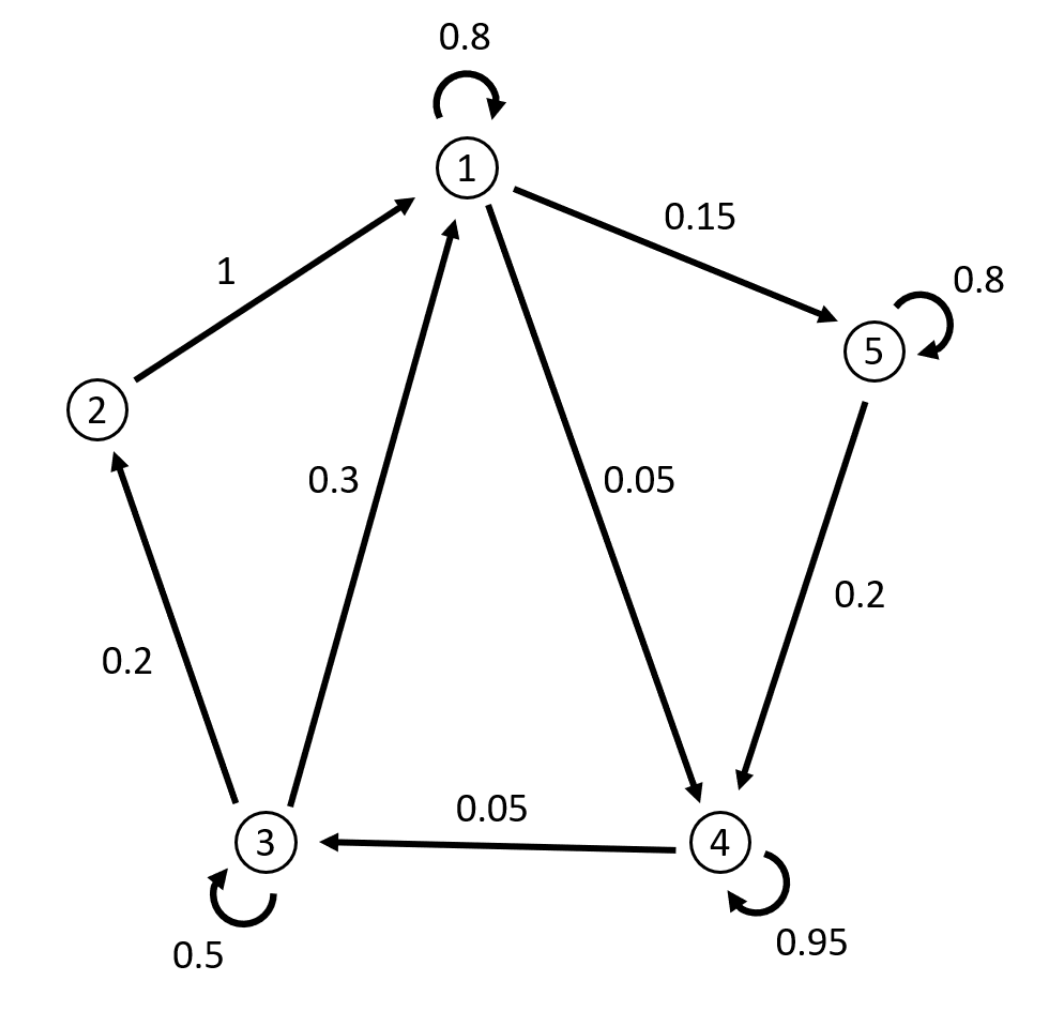
\includegraphics[scale=0.8]{Figure1.1}\\
	Figure 1.1
\end{center}

% Question 1
\begin{enumerate}
	\item Let every node's population be 1 (i.e., $N_i = 1$  for each i). Let  $\beta = 0.8$ and $\gamma = 0.5$. Let all initial infections be 0 except for node 1; node 1's initial infection should be 0.01 (so  $I_i(0)=0.01$ and $S_i(0)=0.99$ , but all other nodes have $S_i(0)=1$,  $I_i(0) = 0$ and $R_i(0) = 0$). What are the S, I, and R quantities after 1 time step?
\end{enumerate}
% Question 1 Answers
\textcolor{gray}{
Answers:
\begin{enumerate}
		\item Letting $t$ denote the current time step we assign this value 1 since that is the time step we are interested in for finding the values of $S_i(t)$, $I_i(t)$, and $R_i(t)$ (when $t=1$).  So, using the equation given to us in class starting from the time step $t=0$ we can find the next time step, $t=1$, with;\\
\textcolor{red}{
\begin{align*}
S_i(t+1) 	&=  S_i(t) - \left(\frac{\beta \times a_{ij} \times S_i(t) \times I_i(t)}{N_i}\right)\\
		&=	S_i(0) - \left(\frac{\beta \times a_{ij} \times S_i(0) \times I_i(0)}{N_i}\right)\\
		&=	1  -\left(\frac{0.8 \times a_{ij} \times 0.99 \times 0.01}{1}\right)\\
\end{align*}
\begin{align*}
I_i(t+1) 	&=  I_i(t) + \left(\frac{\beta \times a_{ij} \times S_i(t) \times I_i(t)}{N_i}\right) - (\gamma I_i(t))\\
		&=	I_i(0) + \left(\frac{\beta \times a_{ij} \times S_i(t) \times I_i(0)}{N_i}\right) - (\gamma I_i(0))\\
		&=	0 + \left(\frac{0..8 \times a_{ij} \times 1 \times 0}{1}\right) - (0.5 \times 0)\\
\end{align*}
\begin{align*}
R_i(t+1) 	&=  R_i(t) + \big(\gamma \times I_i(t)\big)\\
		&=  R_i(0) + \big(\gamma \times I_i(0)\big)\\
		&=  0 + \big(0.5 \times 0 \big)\\
\end{align*}
}
\textcolor{blue}{
\begin{align*}
S_i(t+1) 	&=  S_i(t) \times \left( 1 - \frac{\beta \times a_{ij} \times S_i(t) \times I_i(t)}{N_i}\right)\\
		&=	S_i(0) \times \left( 1 - \frac{\beta \times a_{ij} \times S_i(0) \times I_i(0)}{N_i}\right)\\
		&=	1  \times \left( 1- \frac{0.8 \times a_{ij} \times 0.99 \times 0.01}{1}\right)\\
\end{align*}
\begin{align*}
I_i(t+1) 	&=  I_i(t) + \left(\frac{\beta \times a_{ij} \times S_i(t) \times I_i(t)}{N_i}\right) - (\gamma I_i(t))\\
		&=	I_i(0) + \left(\frac{\beta \times a_{ij} \times S_i(t) \times I_i(0)}{N_i}\right) - (\gamma I_i(0))\\
		&=	0 + \left(\frac{0..8 \times a_{ij} \times 1 \times 0}{1}\right) - (0.5 \times 0)\\
\end{align*}
\begin{align*}
R_i(t+1) 	&=  R_i(t) + \big(\gamma \times I_i(t)\big)\\
		&=  R_i(0) + \big(\gamma \times I_i(0)\big)\\
		&=  0 + \big(0.5 \times 0 \big)\\
\end{align*}
}
\textcolor{green}{
\begin{align*}
S_i(t+1) 	&=  S_i(t) - \sum_{j=0}^{n} \frac{\beta \times a_{ij} \times S_i(t) \times I_i(t)}{N_i}\\
		&=	S_i(0) \times (\beta \times S_i(0)) \times \sum_{j=0}^{n}  a_{ij} \frac{I_i(0)}{N_i}\\
		&=	1 \times (0.8 \times 1) \times \textcolor{orange}{\sum_{j=0}^{n}  a_{ij} \frac{ I_i(0)}{N_i}}\\
\end{align*}
The part of the equation in the orange color can also be described as a matrix with diagnol corresponding values for each iteartion, $n$, 
$\begin{bmatrix} 
	s_1(t) & 0.0  & 0.0 & 0.0 \\
	0.0 & s_2(t)  & 0.0 & 0.0 \\
	0.0 & 0.0  & . . . .  & 0.0 \\
	0.0 & 0.0  & 0.0 & s_n(t) \\
\end{bmatrix}$\\
}
\end{enumerate}
}

% Question 2
\begin{enumerate}
	\setcounter{enumi}{1}
	\item How many time steps would it take before someone is infected in every node?
\end{enumerate}
% Question 2 Answers
\textcolor{gray}{
Answers:
\begin{enumerate}
	\setcounter{enumi}{1}
	\item How many time steps would it take before someone is infected in every node?
\end{enumerate}
}

% Question 3
\begin{enumerate}
	\setcounter{enumi}{2}
	\item Suppose that the connection between node 2 and node 1 is removed. If nothing else changes in the network, would this change the spread of the epidemic? Can you predict how many people in node 2 would eventually get sick?
\end{enumerate}
% Question 3 Answers
\textcolor{gray}{
Answers:
\begin{enumerate}
	\setcounter{enumi}{2}
	\item Suppose that the connection between node 2 and node 1 is removed. If nothing else changes in the network, would this change the spread of the epidemic? Can you predict how many people in node 2 would eventually get sick?
\end{enumerate}
}

% Question 4
\begin{enumerate}
	\setcounter{enumi}{3}
	\item Repeat that same thought experiment, but this time let the initial infection start on node 2 (so $I_2(0) = 0.01$ and $S_2(0) = 0.99$, but all other nodes have $S_i(0)=1$, $I_i(0)=0$  and $R_i(0)=0$). Now can you predict how many people in node 2 would eventually get sick?
\end{enumerate}
% Question 4 Answers
\textcolor{gray}{
Answers:
\begin{enumerate}
	\setcounter{enumi}{3}
	\item Repeat that same thought experiment, but this time let the initial infection start on node 2 (so $I_2(0) = 0.01$ and $S_2(0) = 0.99$, but all other nodes have $S_i(0)=1$, $I_i(0)=0$  and $R_i(0)=0$). Now can you predict how many people in node 2 would eventually get sick?
\end{enumerate}
}

% Question 5
\begin{enumerate}
	\setcounter{enumi}{4}
	\item Instead, suppose you remove the connection from node 2 to node 1, and replace it with a self-loop on 2 with weight 1. If nothing else changes in the network (and the infection starts at node 1), would this change the spread of the epidemic? Can you predict how many people in node 2 would eventually get sick?
\end{enumerate}
% Question 5 Answers
\textcolor{gray}{
Answers:
\begin{enumerate}
	\setcounter{enumi}{4}
	\item Instead, suppose you remove the connection from node 2 to node 1, and replace it with a self-loop on 2 with weight 1. If nothing else changes in the network (and the infection starts at node 1), would this change the spread of the epidemic? Can you predict how many people in node 2 would eventually get sick?
\end{enumerate}
}
\end{document}
